\documentclass[18pt]{beamer}
\usepackage[utf8]{inputenc}
\usepackage{xcolor}
\usepackage{hyperref}
\usepackage{templates/mytemplate}
\usepackage{templates/beamerthemekit}
\usepackage{graphicx}
\usepackage{microtype}
\usepackage{listings}
\usepackage{multicol}
\usepackage{siunitx}
\usepackage{physics}
\usepackage{appendixnumberbeamer}
\usepackage{booktabs}
\usepackage{longtable}
\usepackage{amssymb}
\usepackage{todonotes}

\usepackage{paralist}
\let\itemize\compactitem
\let\description\compactdesc
\let\enumerate\compactenum  

\lstset{ %
  backgroundcolor=\color{white},   % choose the background color; you must add \usepackage{color} or \usepackage{xcolor}; should come as last argument
  basicstyle=\tiny\ttfamily,
  xleftmargin=-10pt,
  breaklines=false,                 % sets automatic line breaking
  captionpos=b,                    % sets the caption-position to bottom
  % frame=single,	                   % adds a frame around the code
  keepspaces=true,                 % keeps spaces in text, useful for keeping indentation of code (possibly needs columns=flexible)
  language=C++,                 % the language of the code
  % morekeywords={*,...},            % if you want to add more keywords to the set
  tabsize=2,	                   % sets default tabsize to 2 spaces
  keywordstyle=\bfseries\color{kit-green70},
  commentstyle=\itshape\color{kit-blue70},
  identifierstyle=\color{black},
  stringstyle=\color{kit-orange100},  
}

\hypersetup{colorlinks=true, urlcolor=kit-blue100, %linkcolor=Firebrick4
}

\title{Estimation of the Track Finding Efficiency using Cosmics Data} 
\subtitle{ETP Belle 2 Weekly Meeting}
\author{\underline{Michael Eliachevitch}}
\date{8 November 2018}
\titleimage{transparent}
\institute{ETP -- KIT}


\begin{document}
\selectlanguage{english}

\section{Introduction}
\begin{frame}
  \titlepage
\end{frame}

\begin{frame}
  \frametitle{Overview}
  \begin{itemize}
  \item look at GCR August cosmics data and new MC with trigger simulation
  \item method to select cosmic events where two track halves are expected
  \item current results 
  \item discussion and outlook
  \end{itemize}
  
\end{frame}

\begin{frame}
  \frametitle{Update on used Cosmics Data and MC}
  \begin{itemize}
  \item last F2F: used data from Juli GCR and my own MC without trigger simulation
  \item \textbf{current data:} GCR August 2017  with single TSF trigger
  \item \textbf{current MC:} GCR August MC ``sample 1'' from DP group: single TSF trigger simulation and narrow acceptbox around IP ($\SI{60}{cm} \times \SI{20}{cm} \times \SI{20}{\cm}$)
    \begin{itemize}
    \item in spite of trigger simulation, track parameter distributions still different  for data and MC due to narrow acceptbox (especially $z_0$)
    \item MC ``sample 2'' with wide acceptbox has become available last week, but could not be analysed until this F2F
    \end{itemize}
  \item Further information on datataking and MC production can be found at the confluence pages for
    \href{https://confluence.desy.de/display/BI/Data+Production+Global+Cosmics+Run+Data\#DataProductionGlobalCosmicsRunData-Runinfo}{data}
    and \href{https://confluence.desy.de/display/BI/Data+Production+Global+Cosmics+Run+MC}{MC}
  \end{itemize}    
\end{frame}

\begin{frame}
  \frametitle{Track Parameter Distributions in August GCR and MC}
  \begin{center}
    \includegraphics[width=0.3\textwidth]{figures/distributions/gcr_august_2017_pt_distribution_normed=True.pdf}
    \includegraphics[width=0.3\textwidth]{figures/distributions/gcr_august_2017_z0_distribution_normed=True.pdf}
    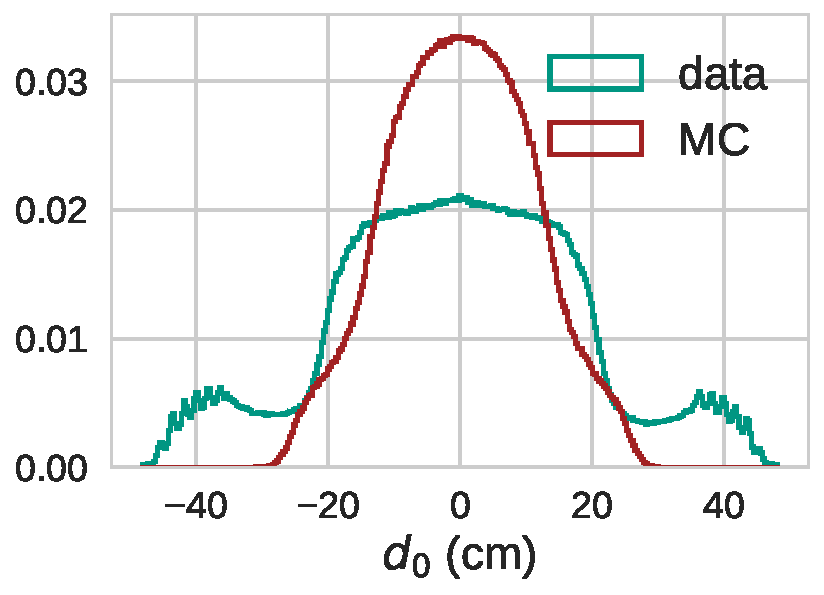
\includegraphics[width=0.3\textwidth]{figures/distributions/gcr_august_2017_d0_distribution_normed=True.pdf}\\
    \includegraphics[width=0.3\textwidth]{figures/distributions/gcr_august_2017_phi0_distribution_normed=True.pdf}
    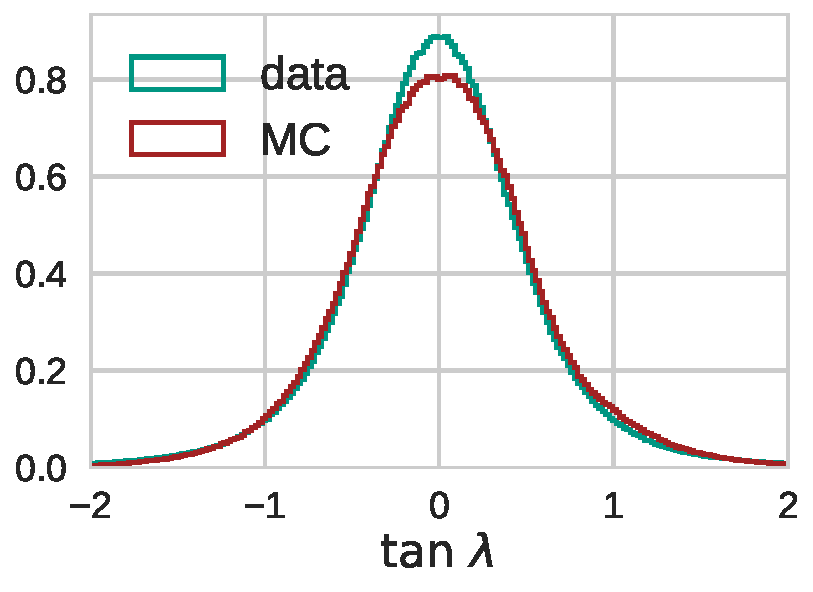
\includegraphics[width=0.3\textwidth]{figures/distributions/gcr_august_2017_tan_lambda_distribution_normed=True.pdf}
  \end{center}
MC generator acceptbox half widths:
    \begin{itemize}
    \item $z:$ 30\,cm
    \item $x, y:$ 10\,cm
    \end{itemize}

\end{frame}
    
\begin{frame}
  \frametitle{Reminder: Estimation of Finding Efficiency}
  \begin{itemize}
  \item typical cosmics event: single muon track, no secondaries
  \item cosmics passing through VXD volume create two \texttt{NonMergedRecoTracks}\\
    $\rightarrow$ in the following use those instead of merged \texttt{RecoTracks}
  \item idea: estimate finding efficiency from \textcolor{kit-red100}{finding fails} in events where \textcolor{kit-blue100}{two (findable) tracks are expected}
  \end{itemize}
  \begin{block}{}
    \begin{equation*}
      \label{eq:cosmic_eff}
      \text{finding efficiency} = \frac{N_\mathrm{2\ tracks\ found}}{\textcolor{kit-blue100}{N_\mathrm{2\ tracks\ expected}}}
      = 1 - \frac{\textcolor{kit-red100}{N_\mathrm{1\ track\ found}}}{\textcolor{kit-blue100}{N_\mathrm{2\ tracks\ expected}}}
    \end{equation*}             %
  \end{block}
  where $\textcolor{kit-red100}{N_\mathrm{1\ track\ found}}, N_\mathrm{2\ tracks\ found}, \in \textcolor{kit-blue100}{N_\mathrm{2\ tracks\ expected}}$.\\
  
  % \includegraphics[width=0.3\textwidth]{figures/b2display_example_1trackevt_cut.png}
\end{frame}

\begin{frame}
  \begin{center}
    \frametitle{Example Finding Fail Event}
    \begin{itemize}
    \item GCR August 2017 data, run 3902, event 13913
    \item \textcolor{kit-blue100}{blue: assigned RecoHits}, \textcolor{kit-red100}{red: unassigned reco hits}
    \item only one reco track found in upper half, finding fail in bottom half
    \end{itemize}
    \includegraphics[width=0.65\textwidth]{figures/b2display_screenshots/gcr_data_2017-08_run3902_evt13913_finding-fail-musterevent.png}
  \end{center}
\end{frame}

\begin{frame}
  \frametitle{Challenges}
  \begin{itemize}
  \item Select set of events with two findable track halves without knowledge of track finding results (e.g. track parameters)
  \item MC Tracks were not split in MC Track Finder, so there was no simple MC truth for the number of tracks
  \item Deal with differences in cosmics data and MC
  \end{itemize}
\end{frame}

\section{Necessary Steps to get the Finding Efficiency}
\begin{frame}
  % Vorgehen / Approach
  \frametitle{Approach}
  \begin{block}{Steps to get the Cosmics based Finding Efficiency}
  \begin{itemize}
  \item Select two datasets based on MC truth where we know that the event contains one / two tracks\\
    $\rightarrow$ use time between \texttt{CDCSimHit}s as MC truth
  \item Based on those, find good parameters to select events with two expected tracks on data. Optimize cuts for high ``purity''
  \item Further refinement: E.g. discard events with unphysical difference in track parameters (e.g. $\Delta p_T$)
  \item In the resulting dataset, count events where only one track was found and create efficiency profiles
  \item Compare this for MC and data and eventually with finding efficency from MC truth matching
  \end{itemize}
\end{block}

\end{frame}


\begin{frame}
  \frametitle{Use hit times for MC truth based selection of events with one or two tracks }
  \begin{itemize}
  \item no MC truth information if there should be one or two \texttt{NonMergedRecoTracks}
  \item use time $\Delta t$ between subsequent \texttt{CDCSimHit}s in \texttt{MCRecoTracks} as MC truth:
    $\text{hit\ distance} \approx c\cdot\Delta t$
  \end{itemize}
  \begin{columns}
    \begin{column}{0.4\textwidth}
      \only<1>{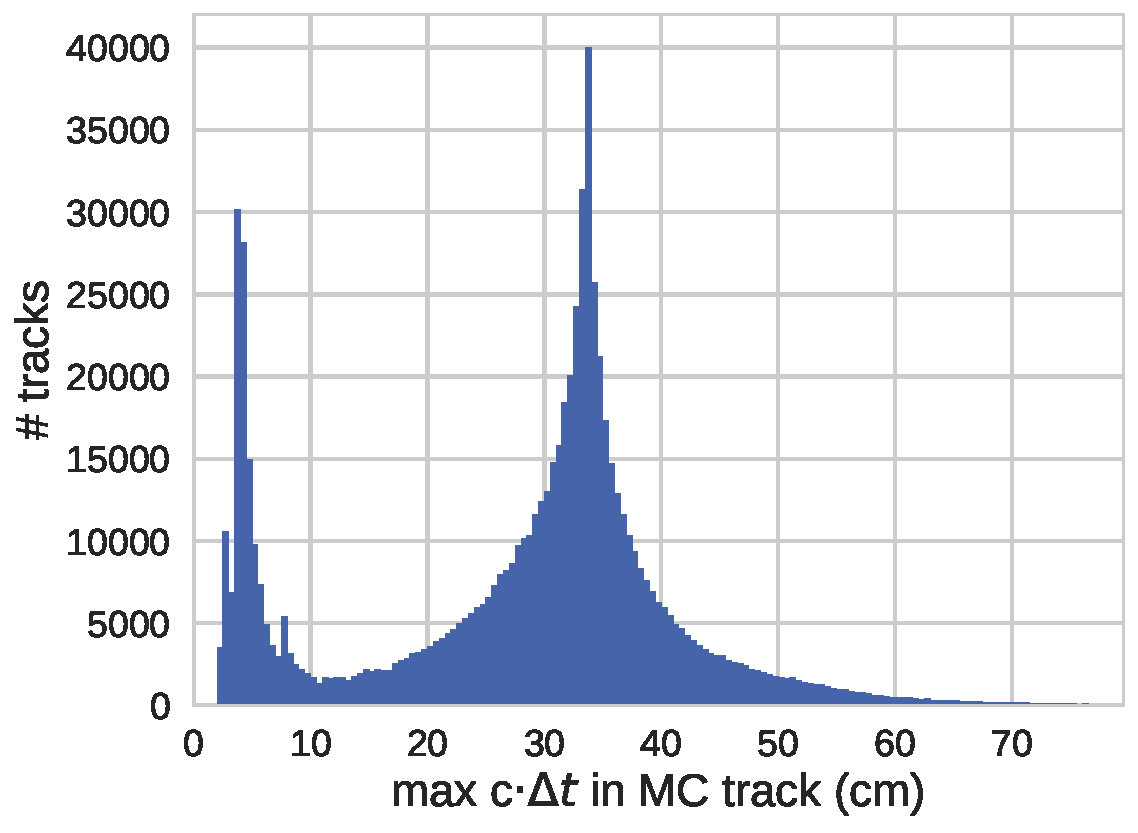
\includegraphics[width=1.\textwidth]{figures/delta_t/gcraugust_delta_t_max_linear_xmin=0.pdf}}
      \only<2->{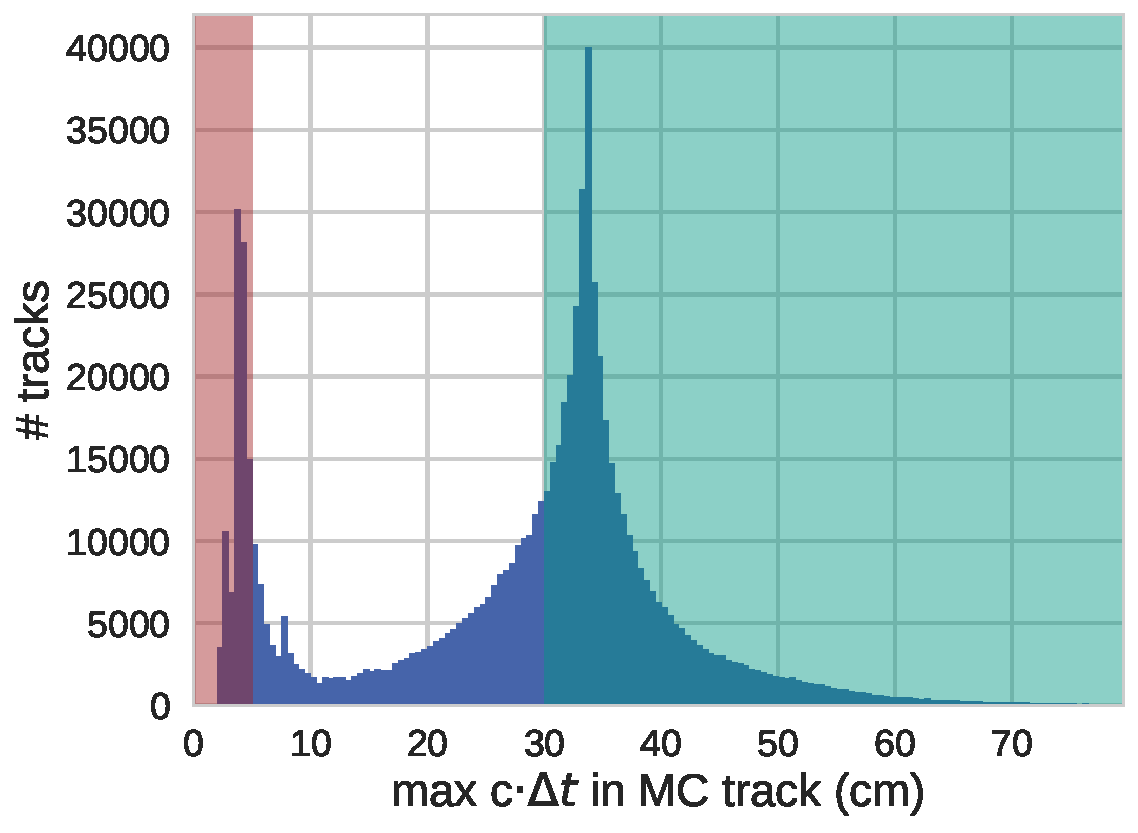
\includegraphics[width=1.\textwidth]{figures/delta_t/gcraugust_delta_t_max_linear_annotated_xmin=0_split=30_maxhitdistance=5.pdf}}
    \end{column}

    \begin{column}{0.35\textwidth}
      \only<2->{
        \begin{itemize}
        \item $(c\Delta t)_\mathrm{max} < \SI{5}{\cm}$:\\\textcolor{kit-red100}{one track expected}
        \item $(c\Delta t)_\mathrm{max} > \SI{30}{\cm}$:\\\textcolor{kit-green100}{two tracks expected}
        \item inbetween: not sure
        \end{itemize}
      }
    \end{column}
    \begin{column}{0.25\textwidth}
      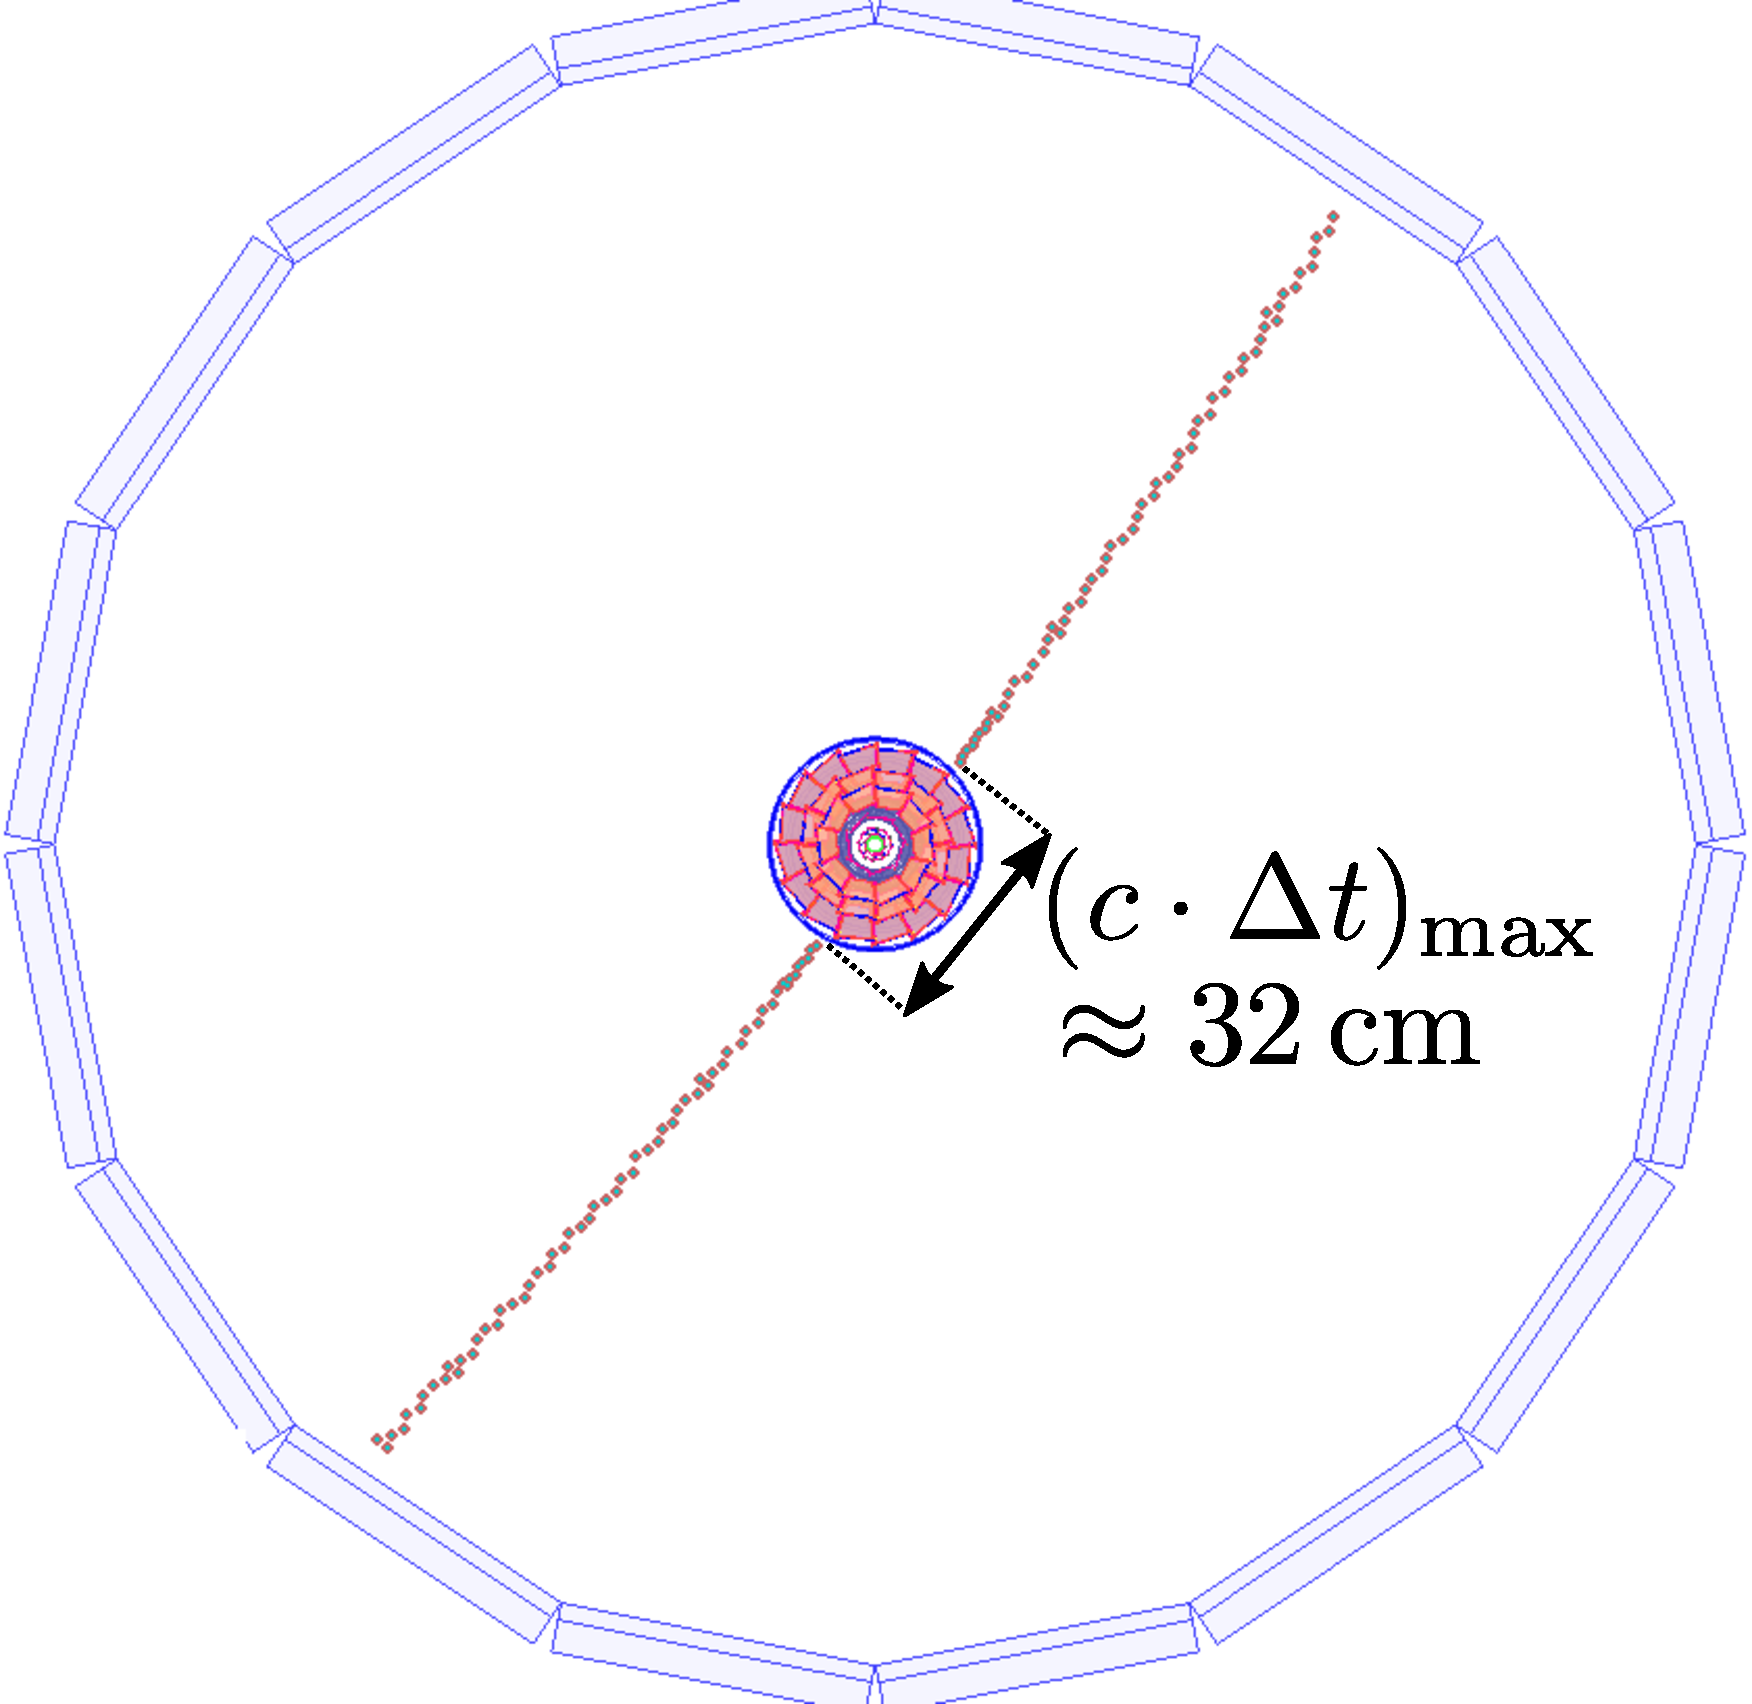
\includegraphics[width=\textwidth]{figures/b2display_screenshots/gcr_mc_2017-08_run4006_evt1_twotrackevent_annotaded.pdf}
    \end{column}
  \end{columns}
\end{frame}




\begin{frame}
  \frametitle{Parameters for selection of  two track events on data}
  Parameters used to select expected two track events on data:
  \begin{itemize}
  \item number of CDC Hits in event
  \item sum of CDCHit y-positions
  \end{itemize}
  \begin{center}
    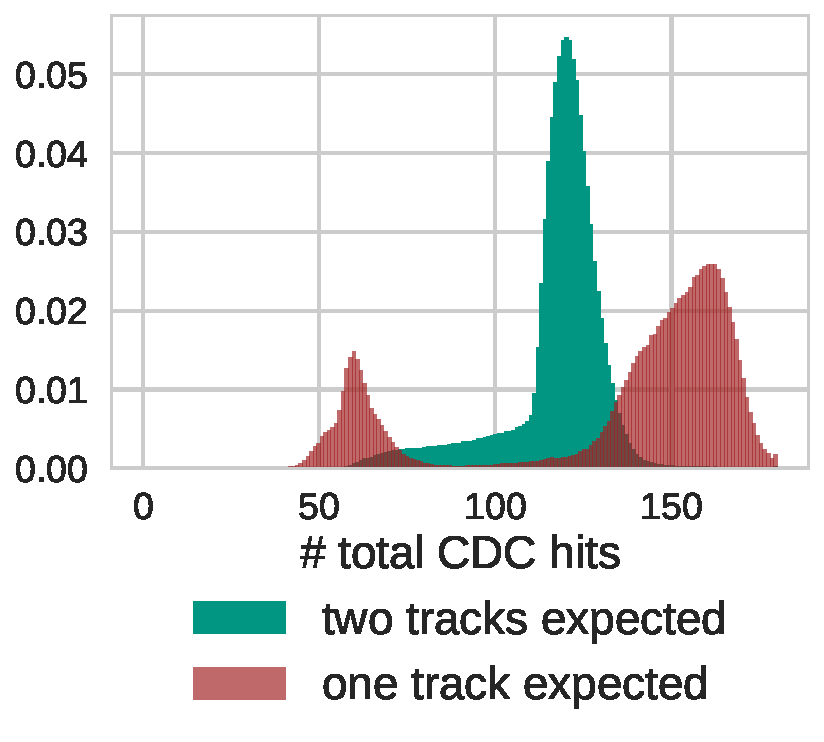
\includegraphics[width=0.45\textwidth]{figures/mcsplit_analysis/total_cdc_hits_gcraugust_30cm_split.pdf}
    \includegraphics[width=0.45\textwidth]{figures/mcsplit_analysis/sum_y_distribution_gcraugust_30cm_split.pdf}
  \end{center}
\end{frame}
  
\begin{frame}
  \begin{center}
    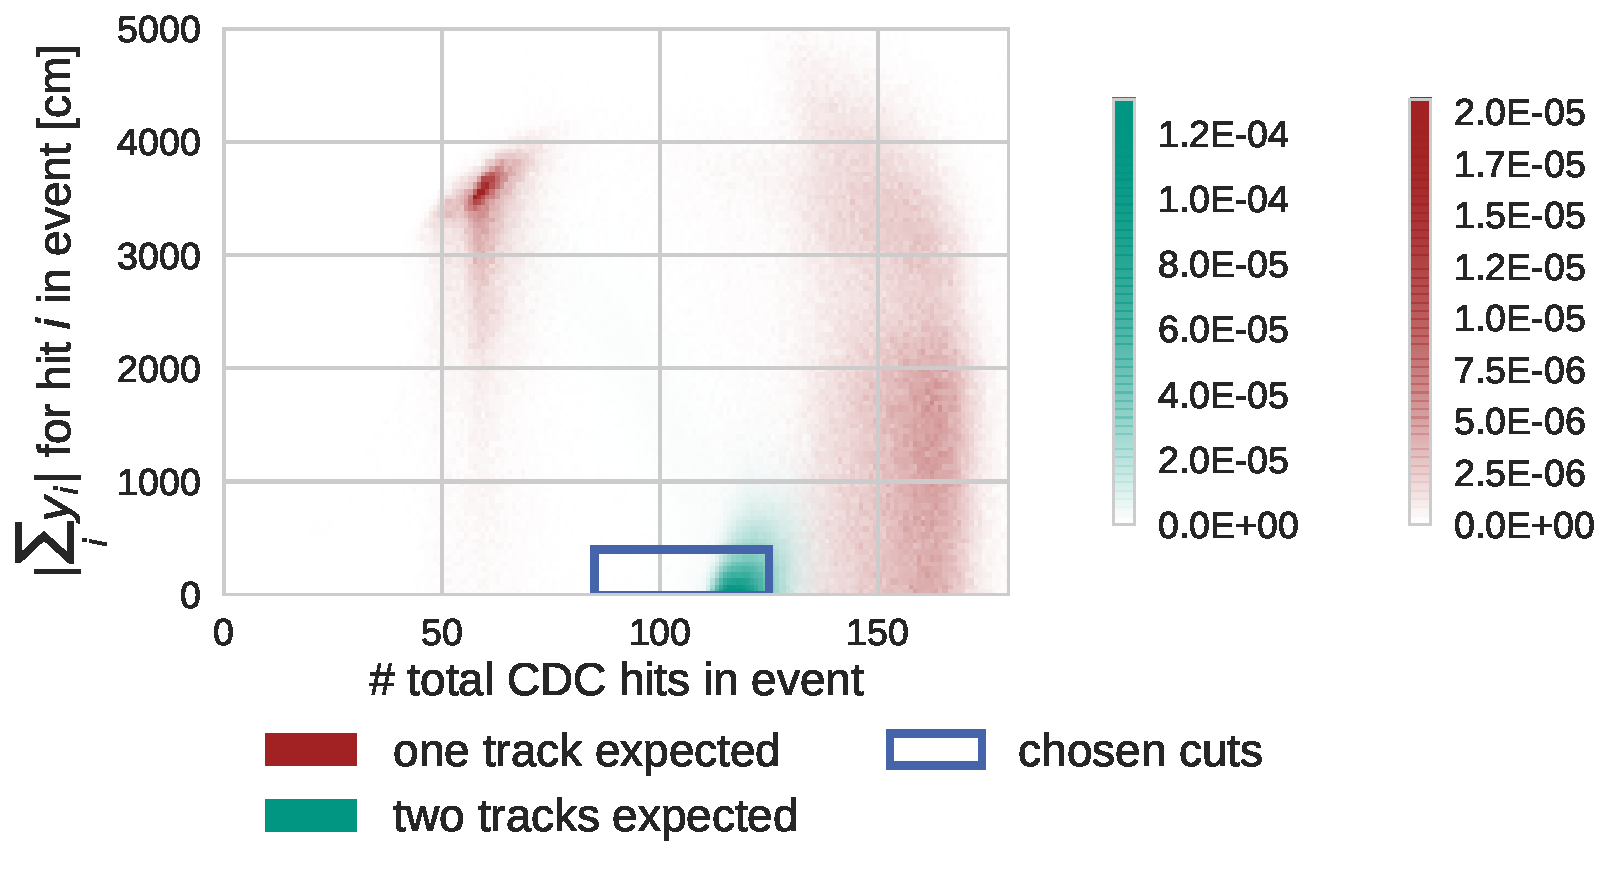
\includegraphics[width=0.72\textwidth]{figures/mcsplit_analysis/sum_y_vs_hits_merged_gcraugust_30cm_split.pdf}
  \end{center}
  \begin{block}{cuts to select two track events on data}
    \begin{itemize}
    \item $85 < \text{number of CDC hits} < 125$
    \item $\abs{\sum{y}} < \SI{400}{\cm}$
    \end{itemize}      
  \end{block}
  \begin{itemize}
    \item \textbf{``purity'': 99.8\%} of 358\,k one track events are not in this cut\\
    \item \textbf{``efficiency'': 43.8\%} of 1.288\,M two track events are in this cut
  \end{itemize}
\end{frame}

\begin{frame}
  \frametitle{Typical examples of excluded one track events}
  
  \begin{columns}
    \begin{column}{0.5\textwidth}
      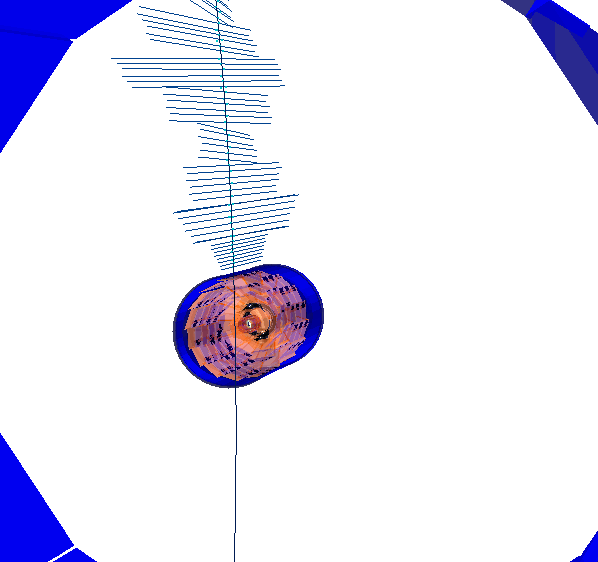
\includegraphics[width=0.7\textwidth]{figures/b2display_screenshots/gcr_2017-08_run4182_evt7_onetrackevent_58cdchits_editet.png}\\
      58 CDC hits, lower than for two track events, because particle stopped at VXD
    \end{column}
    \begin{column}{0.5\textwidth}
      \includegraphics[width=0.7\textwidth]{figures/b2display_screenshots/gcr_2017-08_run4017_evt1_onetrackevent_170cdchits_edited.png}\\
      170 CDC hits, higher than for two track events, because there is no gap around VXD
    \end{column}
  \end{columns}
\end{frame}

\begin{frame}
  \frametitle{Further cuts based on $\Delta p_T$  between the two tracks}
  \begin{itemize}
  \item Aim: exclude events where both found tracks are not related, but from different particles or secondaries
  \item Require that $p_T$ is similar for both tracks. Rough cut: $\abs{\Delta p_T} < \SI{2}{\GeV}$
  \item Problem: Often bad fits due to low hit efficiencies
  \item Highlighted in red and blue: matched hits for first and second track
  \end{itemize}
  \begin{columns}
    \begin{column}{0.5\textwidth}
      \center
      \includegraphics[width=0.45\textwidth]{figures/b2display_screenshots/gcr_data_2017-08_run3912_evt964508_f57_two_unrelated_tracks.png}\\
      two tracks by independent particles
      \\$\Delta p_T \approx \SI{11}{\GeV}$
    \end{column}
    \begin{column}{0.5\textwidth}
      \center
      \includegraphics[width=0.45\textwidth]{figures/b2display_screenshots/gcr_data_2017-08_run3920_evt31009_two_tracks_found_but_bad_fit_r-phi.png}\\
      two tracks by same particle, but only few matched hits in top half, bad fit\\
      $\Delta p_T \approx \SI{17}{\GeV}$
    \end{column}
  \end{columns}
\end{frame}

\begin{frame}
  \frametitle{More insights on $\Delta p_T$ between upper and lower track halves}
  \begin{itemize}    
  \item found bump in data at $\Delta p_T = \SI{0.5}{\GeV}$\\
  \item consistent with MIP energy loss in QCS-R at high $z$ region
  \item bump disappears with cut on $\abs{z_0} < \SI{50}{cm}$, but still does not explain wide $\Delta p_T$ distribution
  \end{itemize}
  \begin{columns}
    \begin{column}{0.45\textwidth}
      \begin{center}
      \includegraphics[width=0.6\textwidth]{figures/efficiency_study/two_track_pt_distance_gcr_august2017_data_mc_z0max=500.pdf}\\
      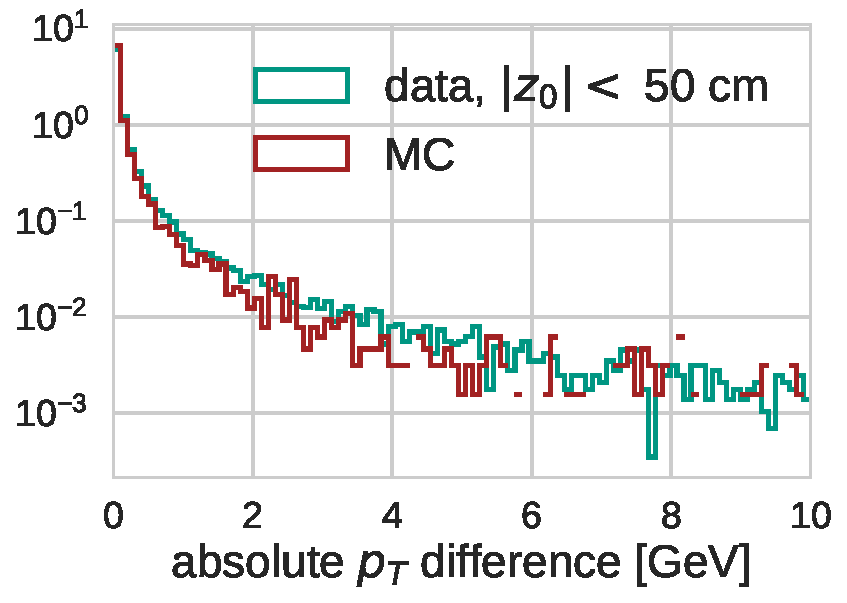
\includegraphics[width=0.6\textwidth]{figures/efficiency_study/two_track_pt_distance_gcr_august2017_data_mc_z0max=50.pdf}
    \end{center}
    \end{column}
    \begin{column}{0.45\textwidth}
      \centering
      \includegraphics[width=1.\textwidth]{figures/efficiency_study/pt_distance_by_z0_gcr_august2017_data.pdf}
    \end{column}    
  \end{columns}
\end{frame}

\begin{frame}
  \frametitle{Types of events where my selection does not work yet}
  \begin{itemize}
  \item looked at events in my selection where only one track was found, expected only finding fails
  \item still often events where there is actually only one findable tracks. Two main types:
  \end{itemize}
  \begin{columns}
    \begin{column}{0.5\textwidth}
      \begin{itemize}
      \item horizontal track $\rightarrow$ small $\sum y$
      \end{itemize}
      \begin{center}
      \includegraphics[width=0.55\textwidth]{figures/b2display_screenshots/gcr_data_2017-08_run3902_evt12895_false-finding-fail_1.png}
    \end{center}

    \end{column}
    \begin{column}{0.5\textwidth}
      \begin{itemize}
      \item cluster with high $\abs{y}$ balances track in other half
      \end{itemize}
      \begin{center}
      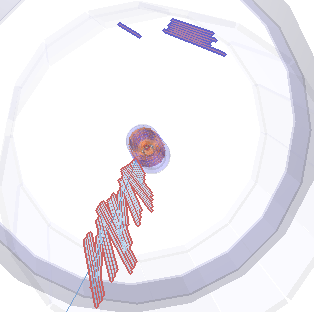
\includegraphics[width=0.55\textwidth]{figures/b2display_screenshots/gcr_data_2017-08_run3902_evt3839_false-finding-fail_2.png}
    \end{center}
    \end{column}
  \end{columns}
    (\textcolor{kit-blue100}{blue: assigned RecoHits}, \textcolor{kit-red100}{red: unassigned reco hits})
\end{frame}


\begin{frame}
  \begin{center}
    \huge Preliminary Results
  \end{center}
\end{frame}

\section{Results}
\begin{frame}
  \begin{block}{All cuts summarized}
    \begin{itemize}
    \item select events where
      \begin{itemize}
      \item $85 < \text{number of CDC hits} < 125$
      \item $\abs{\sum{y}} < \SI{400}{\cm}$
      \end{itemize}
    \item require $\abs{\Delta p_T} < \SI{2}{\GeV}$ for two track events
    \item because MC has narrower $d_0$ and $z_0$ distributions, cut on $\abs{z_0}_\mathrm{max} < \SI{40}{cm}$ and $\abs{d_0}_\mathrm{max} < \SI{20}{cm}$ on MC and data
      to make both distributions more similar
    \end{itemize}
  \end{block}
In the resulting dataset:
  \begin{itemize}
  \item calculate finding efficiency: $N_\mathrm{2\ tracks\ found}/N_\mathrm{2\ tracks\ expected}$
  \item do that also in bins of track parameters (use mean of all tracks)
  \item uncertainties: approximate using poisson error\\
    $\sqrt{N_\mathrm{2\ tracks\ found}}/N_\mathrm{2\ tracks\ expected}$
  \end{itemize}
\end{frame}



\begin{frame}
  \frametitle{Total count and $p_T$ profile}
  \begin{block}{Total count}
  \begin{tabular}{c|cc}
    in selection of events where\\two tracks are expected & GCR August 2017 data &  MC (sample 1)\\
    \hline
    \# one track found & 1281 & 1636 \\
    \# two tracks found &  38851 & 599579\\
    efficiency & 96.8\% & 99.7\% \\
  \end{tabular}
\end{block}
\begin{columns}
  \begin{column}{0.5\textwidth}
    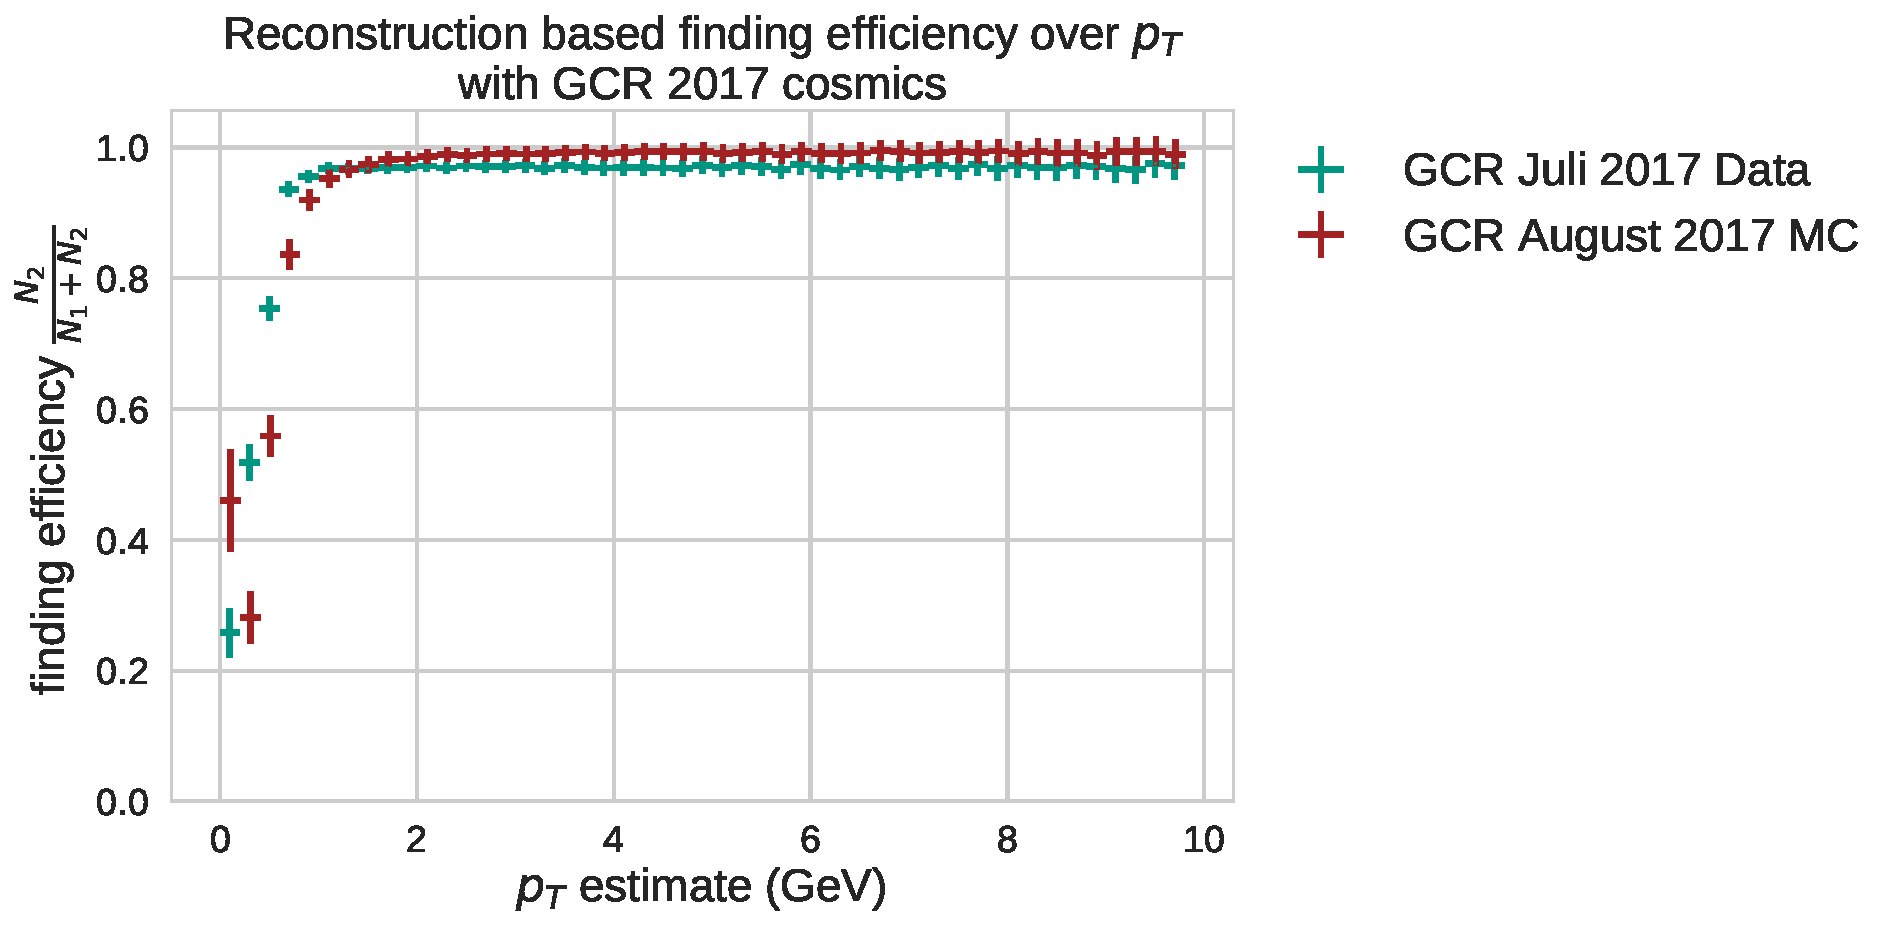
\includegraphics[width=0.85\textwidth]{figures/efficiency_study/cosmicbased_findeff_over_pt.pdf}
  \end{column}
  \begin{column}{0.5\textwidth}
    \begin{itemize}
    \item $>$ 1\,GeV very few finding fails
    \item at low $p_T$ steep decrease: bad efficiency or breakdown of method?
    \item MC slightly better than data, especially at low $p_T$
    \end{itemize}
  \end{column}
\end{columns}
\end{frame}

\begin{frame}
  \frametitle{Profiles by other track parameters}
  \begin{columns}
    \begin{column}{0.5\textwidth}
      \centering
      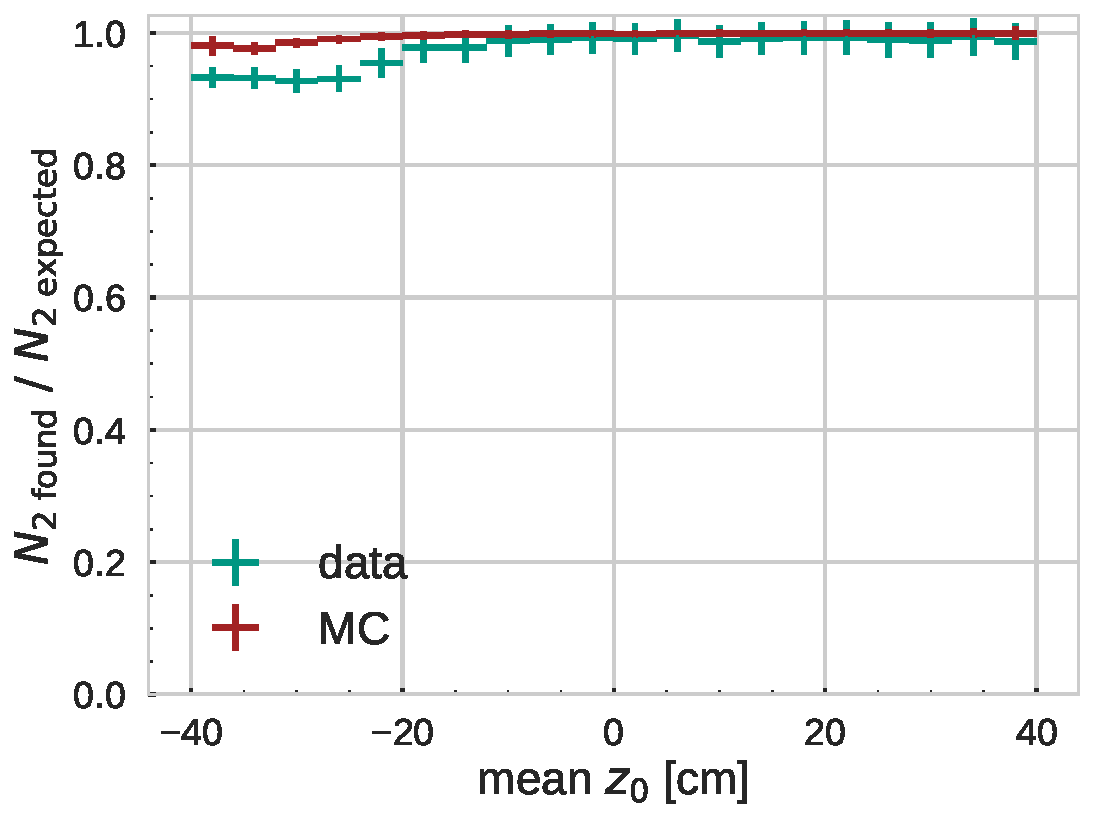
\includegraphics[width=0.85\textwidth]{figures/efficiency_study/cosmicbased_findeff_over_z0.pdf}\\
      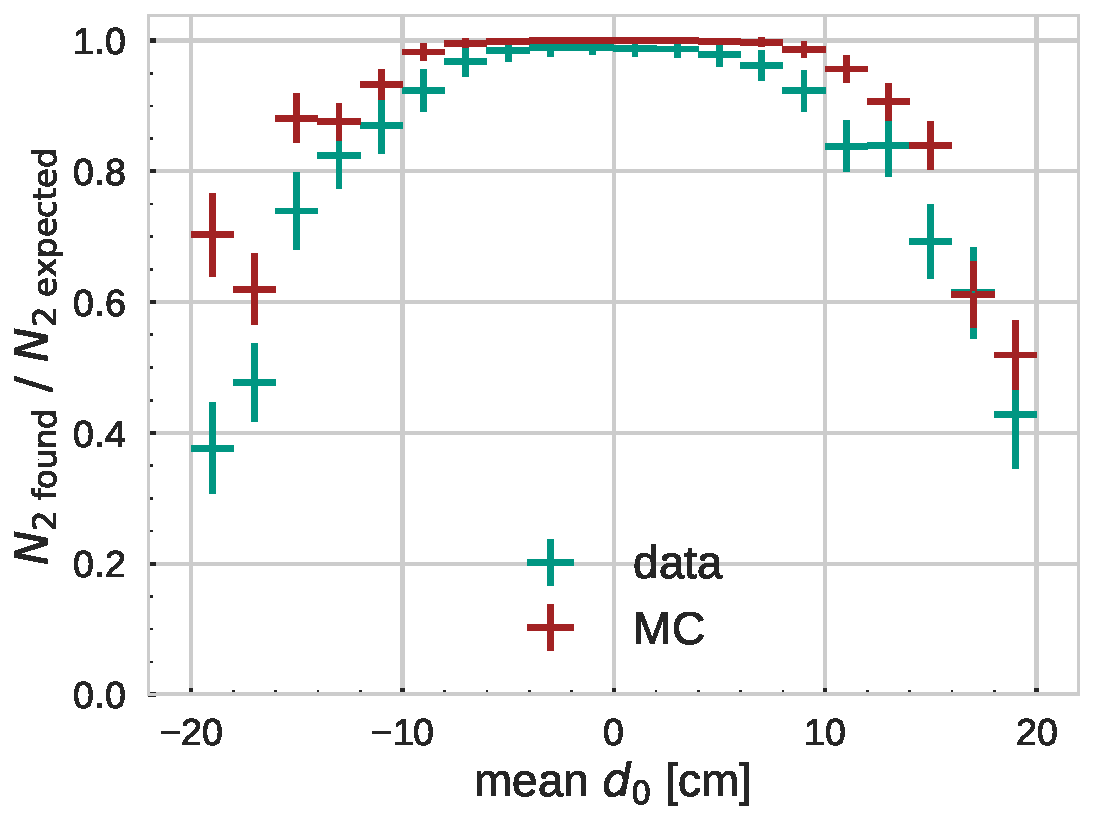
\includegraphics[width=0.85\textwidth]{figures/efficiency_study/cosmicbased_findeff_over_d0.pdf}
      
    \end{column}
    \begin{column}{0.5\textwidth}
      \centering
      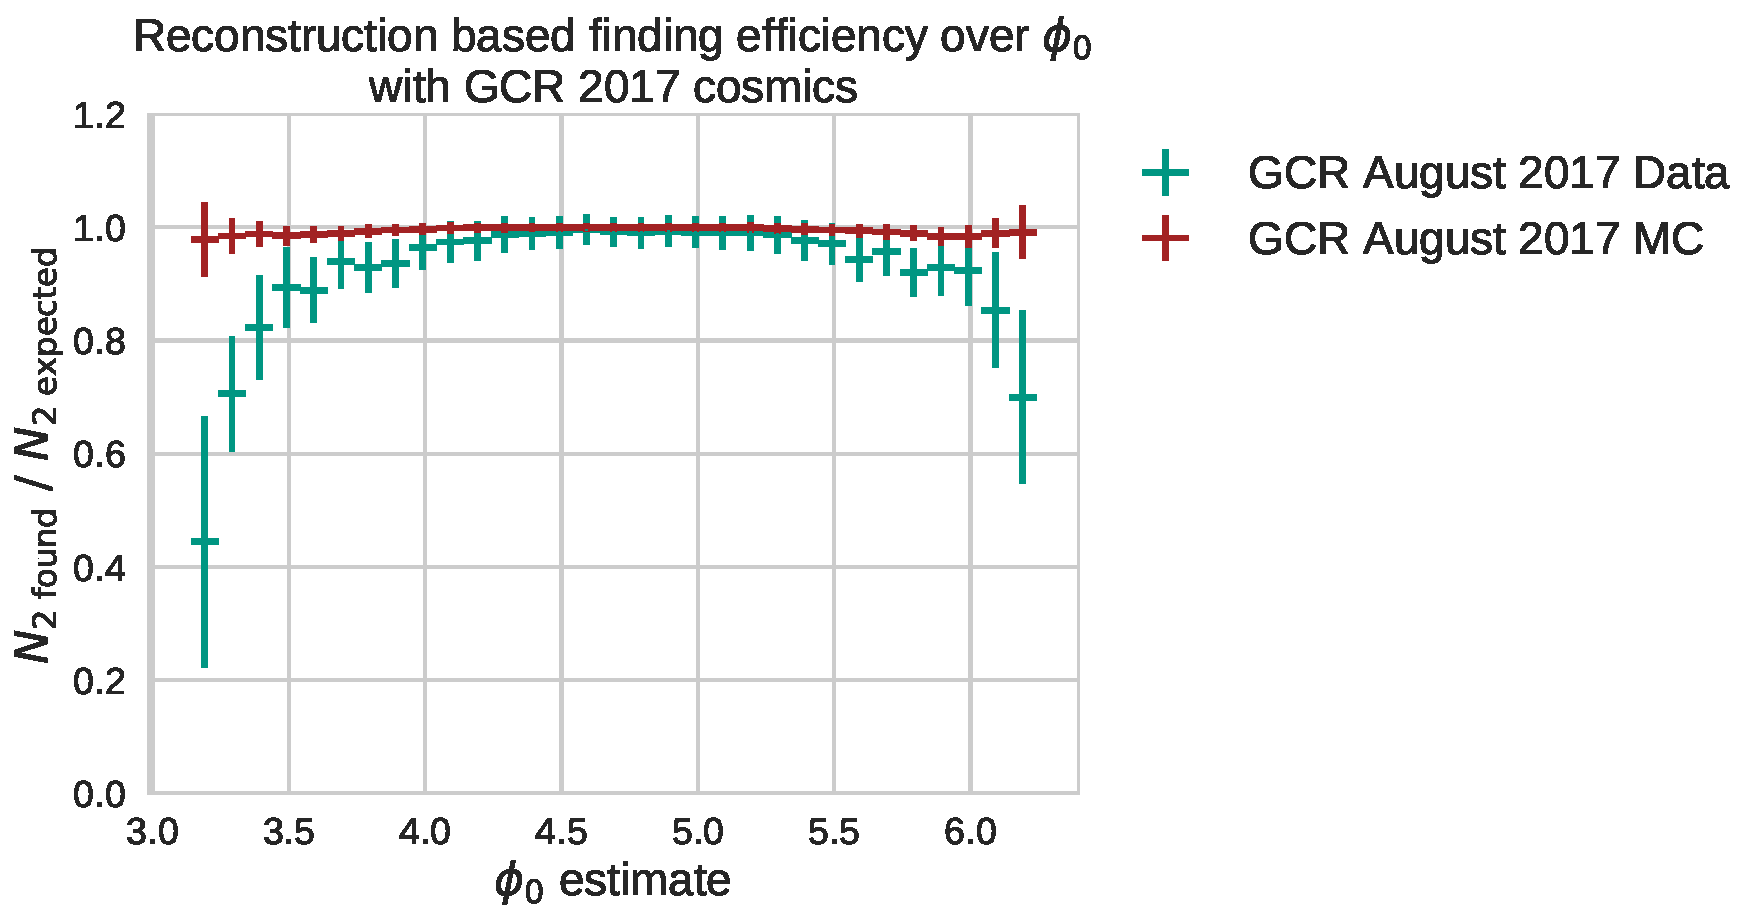
\includegraphics[width=0.85\textwidth]{figures/efficiency_study/cosmicbased_findeff_over_phi0.pdf}\\
      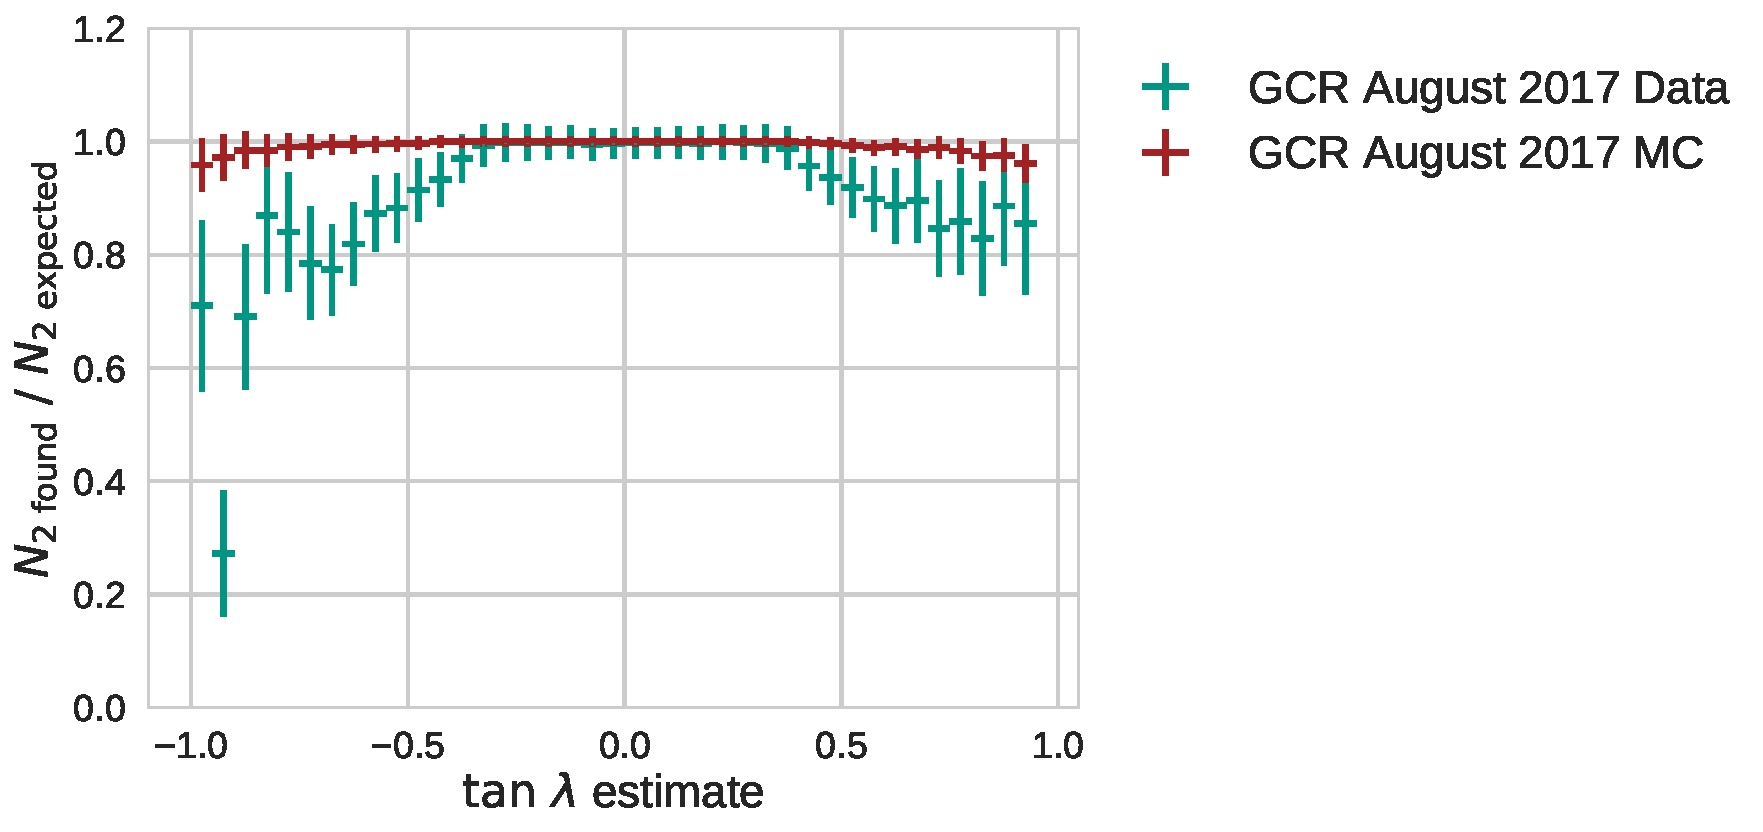
\includegraphics[width=0.85\textwidth]{figures/efficiency_study/cosmicbased_findeff_over_tan_lambda.pdf}
    \end{column}
  \end{columns}
\end{frame}

\begin{frame}
  \frametitle{Discussion of my Results}
  \begin{itemize}
  \item GOOD: Generally, finding fails very rare\\
    $\rightarrow$  \textbf{Confirmation that tracking works on on real data!}
  \item Many events where only one track is found are in low $p_T$ regions and extreme track parameter regions.
    In these regions are large differences between MC and data
  \item Cuts based on $\sum y$ assume almost straight track coming from above. We have seen that this does not always work, which might explain this low ``efficiencies'' in these regions.
  \item Seen in event displays and track parameter differences between both track halves:
    Often bad hit efficiencies and bad fit results. Only due to use of only half lengths (Glückstern Formula)?
  \end{itemize}
  
\end{frame}

\begin{frame}
  \frametitle{Outlook}
  \begin{itemize}
  \item Increase trust on selection of events where we expect two tracks
    \\$\rightarrow$ further cuts?
  \item Compare with finding efficiency from MC matching? Difficult, because it works only well for merged tracks.
  \item Use new GCR MC sample with large 8\,m acceptox. Do differences between MC and data remain?
  \item Use cosmics to estimate hit efficiency. Create efficiency map?
  \end{itemize}
\end{frame}

\section{Backup}

\begin{frame}
  \begin{center}
    \huge Backup
  \end{center}
\end{frame}

\begin{frame}
  \frametitle{More on QCS-R Geometry and $p_T$ difference}
  \includegraphics[width=0.4\textwidth]{figures/efficiency_study/pt_distance_by_z0_gcr_august2017_data.pdf}
  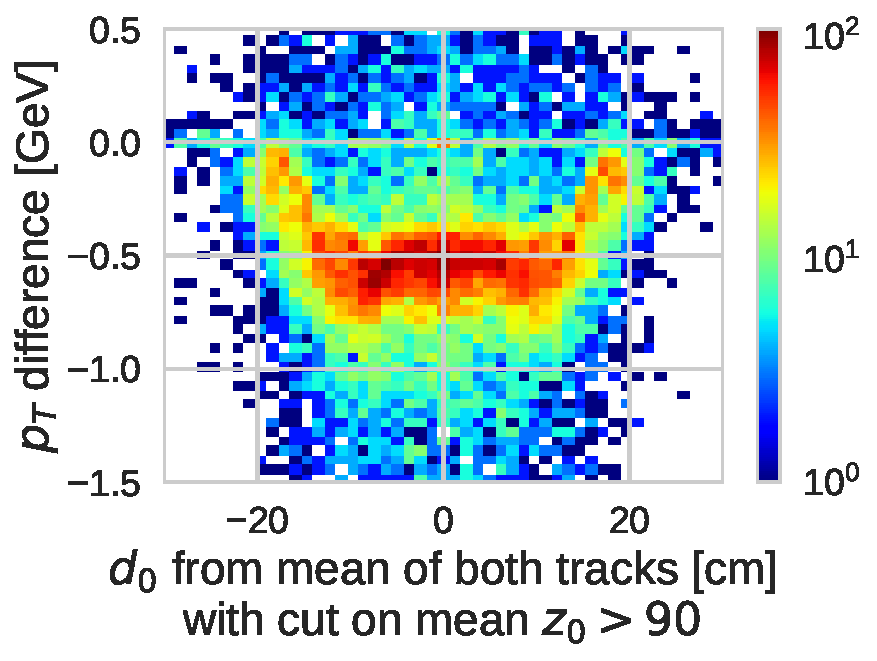
\includegraphics[width=0.4\textwidth]{figures/efficiency_study/pt_distance_by_d0_gcr_august2017_data.pdf}\\
  \begin{center}
    \includegraphics[width=0.4\textwidth]{figures/QCS-R.png}\\
    \scriptsize{(from Belle 2 Design Report 2010)}
  \end{center}
\end{frame}


\begin{frame}
  \frametitle{Distribution of Hit $\Delta t$ for all hits in all tracks}  
  \begin{center}
    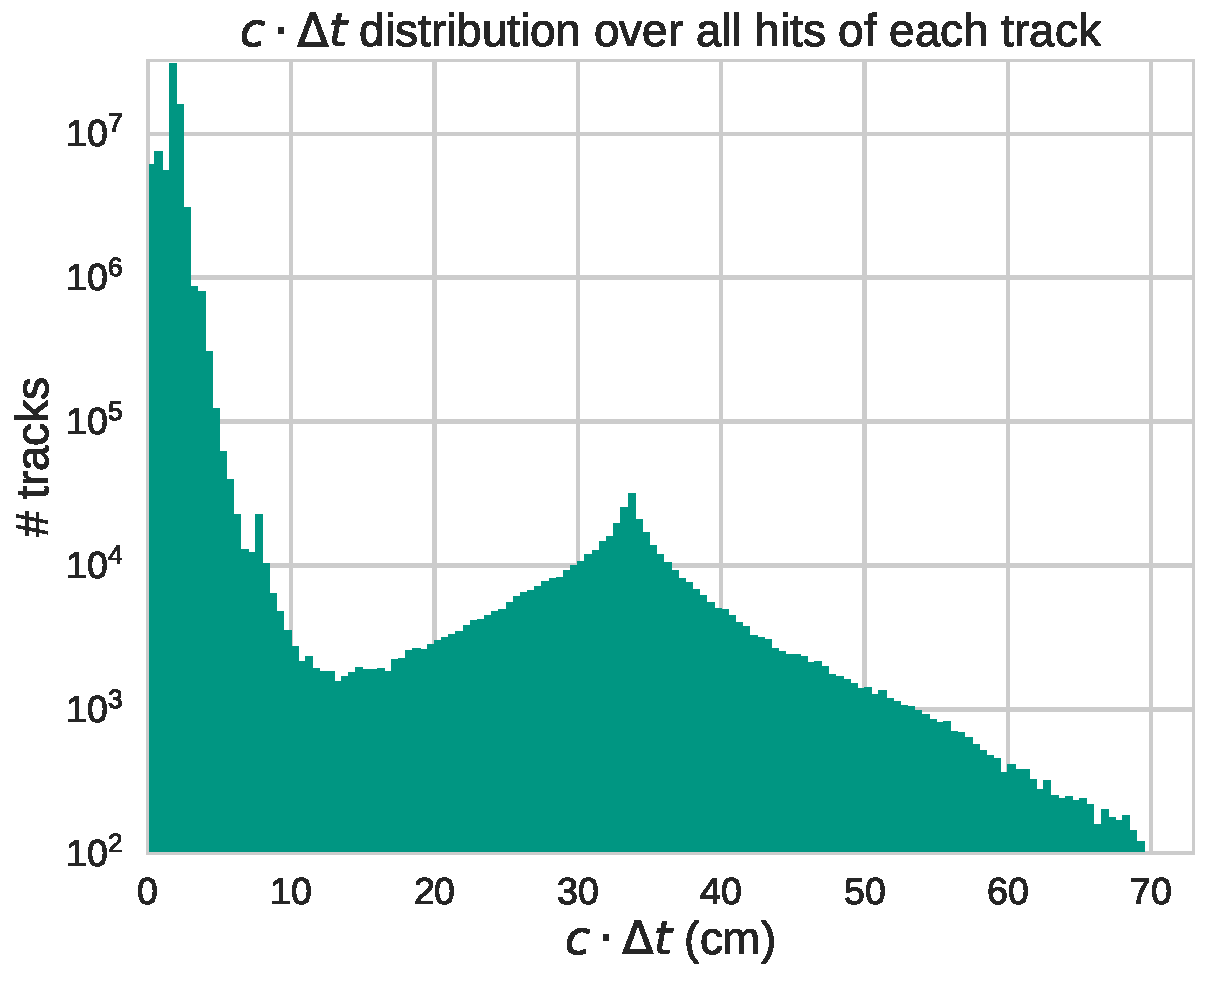
\includegraphics[width=0.45\textwidth]{figures/delta_t/gcraugust_delta_t_log.pdf}
  \end{center}
\end{frame}

\begin{frame}
  \frametitle{VXD dimensions}
  \includegraphics[width=0.8\textwidth]{figures/vxd_dimensions.pdf}\\
  Taken from Belle 2 technical design report (2010). All dimensions are given in mm.
\end{frame}

\begin{frame}
  \frametitle{Kinematic Distributions for Juli GCR}
  Data from Juli 2017 GCR and MC without trigger simulation
  \begin{center}
    \includegraphics[width=0.3\textwidth]{figures/distributions/gcr_juli_2017_pt_distribution_normed=True.pdf}
    \includegraphics[width=0.3\textwidth]{figures/distributions/gcr_juli_2017_z0_distribution_normed=True.pdf}
    \includegraphics[width=0.3\textwidth]{figures/distributions/gcr_juli_2017_d0_distribution_normed=True.pdf}\\
    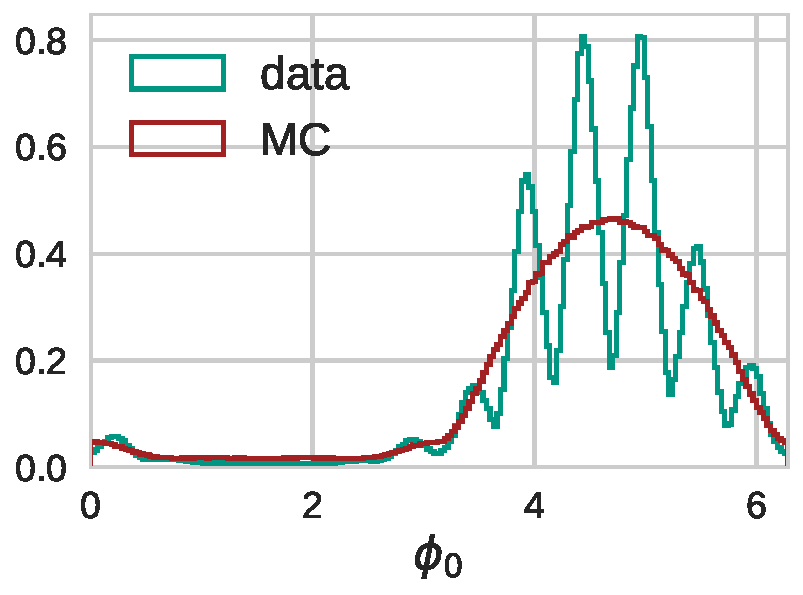
\includegraphics[width=0.3\textwidth]{figures/distributions/gcr_juli_2017_phi0_distribution_normed=True.pdf}
    \includegraphics[width=0.3\textwidth]{figures/distributions/gcr_juli_2017_tan_lambda_distribution_normed=True.pdf}
  \end{center}
\end{frame}
  
\begin{frame}[fragile]
  \frametitle{Code for Splitting Tracks in MC Track Finder}
\begin{lstlisting}[language=C++]
std::vector< std::vector<TimeHitIDDetector> > hitsWithTimeAndDetectorInformationVectors;

if (m_splitAfterDeltaT < 0.0) { // no splitting, vector will only contain a single hitInformation vector
  hitsWithTimeAndDetectorInformationVectors.push_back(hitsWithTimeAndDetectorInformation);
} else { // split on delta t

  std::vector<TimeHitIDDetector>::size_type splitFromIdx = 0; // whenever splitting subtrack, start slice from this index
  for (std::vector<TimeHitIDDetector>::size_type i = 1; i != hitsWithTimeAndDetectorInformation.size(); i++) {

    double delta_t = (std::get<0>(hitsWithTimeAndDetectorInformation[i])
                      - std::get<0>(hitsWithTimeAndDetectorInformation[i - 1]));

    if (delta_t > m_splitAfterDeltaT) {
      // push slice of `hitsWithTimeAndDetectorInformation' between splitFromidx  and previous index
      hitsWithTimeAndDetectorInformationVectors
      .emplace_back(hitsWithTimeAndDetectorInformation.begin() + splitFromIdx,
                    hitsWithTimeAndDetectorInformation.begin() + i);
      splitFromIdx = i;
    }
  }
  // add subtrack after last splitting to list of tracks
  hitsWithTimeAndDetectorInformationVectors
  .emplace_back(hitsWithTimeAndDetectorInformation.begin() + splitFromIdx,
                hitsWithTimeAndDetectorInformation.end());
}
\end{lstlisting}
\end{frame}


\end{document}

%%% Local Variables:
%%% mode: latex
%%% TeX-master: t
%%% End:
